\documentclass[../tesis.tex]{subfiles}
\begin{document}

\chapter{Metodología}
\label{cap:metodologia}

Este capítulo describe el marco metodológico diseñado para abordar el problema de investigación y comprobar las hipótesis planteadas. Se detalla el diseño del estudio, el flujo de procesamiento de datos (\textit{pipeline}), el entrenamiento de la escalera de algoritmos de aprendizaje automático y el esquema de validación estadística e interpretabilidad. Finalmente, se presenta el cronograma de trabajo estipulado para la ejecución del proyecto.

% ─────────────────────────────────────────────────────────────────────────────
\section{Diseño de la investigación}
\label{sec:diseno_investigacion}
% ─────────────────────────────────────────────────────────────────────────────

El presente estudio se clasifica como una investigación analítica retrospectiva basada en datos secundarios. Utiliza como fuente primaria la base de datos longitudinal del Centro de Investigación en Movimiento Humano (CIMOHU) de la Universidad de Costa Rica \cite{CIMOHUdb2026}. El \textit{pipeline} metodológico se divide en cuatro fases secuenciales que abarcan desde la consolidación del \textit{dataset} hasta la validación clínica de los modelos predictivos, como se ilustra en la Figura~\ref{fig:pipeline}.

\begin{figure}[h]
\centering
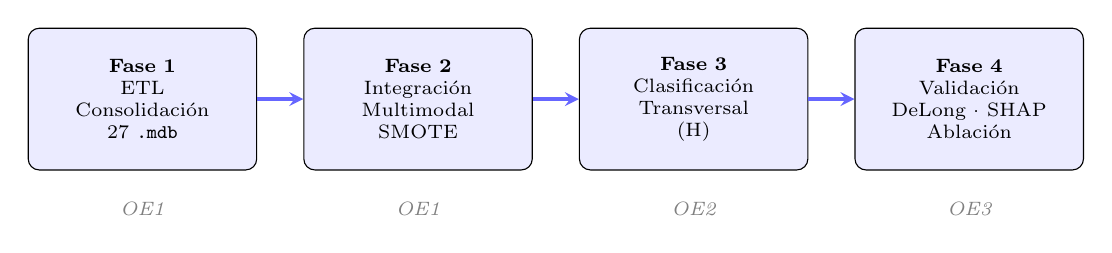
\begin{tikzpicture}[
  phase/.style={draw, rounded corners=4pt, text width=2.55cm, align=center,
                font=\scriptsize, inner sep=5pt, minimum height=1.8cm,
                fill=blue!8},
  arrow/.style={->, very thick, >=stealth, color=blue!60},
  label/.style={font=\scriptsize\itshape, text=gray}
]
  \node[phase] (f1) at (0,0)   {\textbf{Fase 1} \\ ETL \\ Consolidación \\ 27 \texttt{.mdb}};
  \node[phase] (f2) at (3.5,0) {\textbf{Fase 2} \\ Integración \\ Multimodal \\ SMOTE};
  \node[phase] (f3) at (7.0,0) {\textbf{Fase 3} \\ Clasificación \\ Transversal \\ (H)};
  \node[phase] (f4) at (10.5,0) {\textbf{Fase 4} \\ Validación \\ DeLong · SHAP \\ Ablación};

  \draw[arrow] (f1) -- (f2);
  \draw[arrow] (f2) -- (f3);
  \draw[arrow] (f3) -- (f4);

  \node[label] at (0,-1.4)    {OE1};
  \node[label] at (3.5,-1.4)  {OE1};
  \node[label] at (7.0,-1.4)  {OE2};
  \node[label] at (10.5,-1.4) {OE3};
\end{tikzpicture}
\caption[\textit{Pipeline} metodológico de cuatro fases]{\textit{Pipeline} metodológico de cuatro fases. Cada fase corresponde a uno o más objetivos específicos (OE) de la investigación. Las fases se ejecutan secuencialmente; los resultados de cada fase son la entrada de la siguiente.}
\label{fig:pipeline}
\end{figure}

% ─────────────────────────────────────────────────────────────────────────────
\section{Fase 1: Consolidación y preprocesamiento (\textit{ETL})}
\label{sec:fase1_etl}
% ─────────────────────────────────────────────────────────────────────────────

La primera fase consiste en la extracción, transformación y carga (ETL) de los datos crudos. El equipo DXA (GE Lunar Prodigy) del CIMOHU ha generado 27 respaldos históricos en formato \texttt{.mdb} a lo largo de 17 años (2009--2026).

\begin{itemize}
    \item \textbf{Consolidación:} Se migrarán y unificarán los 27 respaldos hacia una base de datos relacional robusta (SQLite, \texttt{prodigy.db}), integrando un total de 9.426 exámenes correspondientes a los 3.240 pacientes adultos registrados (3.231 con al menos un examen).
    \item \textbf{Control de calidad y limpieza:} Se aplicará la de-duplicación por identificador de paciente (\texttt{patient\_id}) y fecha. Se validarán los rangos clínicos permisibles (e.g., valores de DMO positivos, T-scores entre $-6$ y $+6$) para aislar posibles artefactos o \textit{drift} instrumental. La fidelidad instrumental del equipo GE Lunar Prodigy del CIMOHU ha sido validada localmente por \textcite{ChaconAraya2024}, quienes reportaron coeficientes de variación test-retest sumamente bajos (0,17\,\%--3,76\,\%), estableciendo un piso de reproducibilidad robusto para la extracción de características.
    \item \textbf{Imputación de datos:} Dada la naturaleza de los estudios retrospectivos, variables multimodales específicas como el Análisis Estructural de Cadera (HSA) y la Morfometría Vertebral (VFA) presentan valores faltantes. Se utilizarán técnicas de imputación múltiple por ecuaciones encadenadas (MICE) y análisis de sensibilidad para el manejo de estos vacíos.
    \item \textbf{Descarte de la variable ``Etnia'':} Se elimina explícitamente la columna \texttt{ethnicity} del conjunto de datos. El 98{,}5\,\% de los pacientes figuran como ``White'', un valor por defecto del software GE Lunar Prodigy que no representa la demografía costarricense real; conservarla introduciría ruido y sesgo en cualquier modelo predictivo.
    \item \textbf{Corrección del identificador de composición corporal de cuerpo completo:} La extracción de las variables de composición corporal (masa grasa, masa magra, masa ósea) se realizará filtrando estrictamente por \texttt{site=13} \textbf{y} \texttt{label=61} en la tabla \texttt{lunar\_\_Composition}. El identificador \texttt{label=100}, utilizado erróneamente en una versión previa del \textit{pipeline}, mezcla regiones parciales de cadera y columna, generando magnitudes sin sentido físico (decenas a cientos de gramos en lugar de las decenas de miles esperadas para un escaneo de cuerpo completo).
    \item \textbf{Exclusión de variables con fuga de información (\textit{data leakage}):} Tanto los T-scores como la densidad ósea cruda (\texttt{bmd\_total}) quedan excluidos, de forma explícita y permanente, del conjunto de variables predictoras de entrada ($X$) en todas las fases posteriores, dado que la etiqueta objetivo ($Y$, clasificación OMS de osteoporosis) se deriva matemáticamente de ellos.
\end{itemize}

% ─────────────────────────────────────────────────────────────────────────────
\section{Fase 2: Integración multimodal y manejo de desbalance}
\label{sec:fase2_multimodal}
% ─────────────────────────────────────────────────────────────────────────────

\textbf{Reestructuración por exclusión mutua de cohortes.} La base CIMOHU presenta una limitación estructural crítica: la cohorte de pacientes con T-score válido de columna y/o cadera (\texttt{site} $\in \{0,1,2,3\}$; $n = 2.591$) y la cohorte con escaneo de cuerpo completo que permite extraer composición corporal (\texttt{site=13} \textbf{y} \texttt{label=61}, con masas estrictamente positivas; $n = 665$) son \textbf{casi mutuamente excluyentes}: únicamente 42 pacientes coinciden en ambas cohortes. (La auditoría general de la base de datos, sin el filtro de masas positivas aplicado en el \textit{pipeline} de modelado, reporta 668 pacientes con al menos un registro de \texttt{site=13}/\texttt{label=61}; la diferencia de 3 pacientes corresponde a registros con masas nulas o negativas excluidos por control de calidad, véase §~\ref{sec:fase1_etl}.) En consecuencia, no es viable fusionar todas las modalidades en un único \textit{dataset} multimodal por paciente sin recurrir a una imputación masiva ($\sim$99\,\%) de las variables de composición corporal dentro de la cohorte etiquetada, imputación que no aportaría señal real al modelo.

Ante esta restricción, el diseño se reestructura como un \textbf{análisis de ablación con dos modelos separados} en lugar de un modelo único totalmente fusionado:
\begin{itemize}
    \item \textbf{Modelo principal (H):} entrenado sobre la cohorte etiquetada ($n = 2.591$) con las modalidades DMO, demografía y HSA. Es el modelo evaluado formalmente contra los comparadores clínicos en la Fase~4.
    \item \textbf{Modelo secundario (ablación de composición corporal):} entrenado sobre la intersección real de ambas modalidades a nivel de paciente ($n = 42$: pacientes con T-score válido \textbf{y} escaneo de cuerpo completo con composición corporal, filtrando estrictamente \texttt{site=13} y \texttt{label=61}, véase §~\ref{sec:fase1_etl}), para medir de forma aislada el aporte del tejido blando (masa grasa y masa magra) sobre la densidad ósea.
\end{itemize}

\textbf{Reformulación del modelo secundario como tarea de regresión.} La auditoría numérica de la cohorte piloto (§~\ref{sec:resultados_pilotob}) reveló que los 42 pacientes de la intersección real presentan \textbf{cero casos de osteoporosis} (T-score peor observado $= -2{,}10$, por encima del umbral OMS de $-2{,}5$). Este hallazgo no es un artefacto muestral aleatorio, sino la manifestación de un \textbf{sesgo demográfico estructural del CIMOHU}: los pacientes que se someten a un escaneo de composición corporal de cuerpo completo acuden mayoritariamente por indicación deportiva o nutricional, y constituyen una subpoblación sistemáticamente más joven y sana que la cohorte clásica de referencia para osteoporosis. Con una sola clase presente, la tarea de \textbf{clasificación binaria es matemáticamente inviable} sobre esta intersección (AUC-ROC, sensibilidad y especificidad quedan indefinidos). En consecuencia, el modelo secundario se reformula como una \textbf{tarea de regresión continua sobre el T-score} (\texttt{tscore\_min}), que sí posee varianza suficiente en esta sub-cohorte (rango observado $\approx -2{,}10$ a $+4{,}36$), en lugar de una clasificación Normal/Osteoporosis.

\textbf{Validación cruzada Leave-One-Out (LOOCV).} Dado el tamaño de muestra reducido de esta sub-cohorte ($n = 42$), un único \textit{holdout} 80/20 dejaría apenas $\sim$8 pacientes en el conjunto de prueba, una base estadísticamente insuficiente para estimar el poder predictivo del modelo. Por ello, el modelo secundario se evalúa mediante \textbf{Validación Cruzada Leave-One-Out} (\textit{Leave-One-Out Cross-Validation}, LOOCV), en la que cada uno de los 42 pacientes se predice a partir de un modelo entrenado con los 41 restantes. LOOCV constituye el estándar estadístico riguroso para muestras reducidas, ya que maximiza el uso de los datos disponibles para el entrenamiento en cada iteración y produce una estimación del error de generalización con varianza mínima entre pliegues. El desempeño se reporta mediante el coeficiente de determinación ($R^2$) y el Error Absoluto Medio (MAE) promediados sobre las 42 predicciones fuera de muestra.

\textbf{Limitación cuantificada --- multicolinealidad severa de las variables de composición corporal.} El porcentaje de grasa corporal (\texttt{percent\_fat\_bodycomp}) se calcula como una función determinística de la masa grasa y la masa magra: $\%\text{grasa} = \text{grasa} / (\text{grasa} + \text{magra} + \text{ósea}) \times 100$. Incluir simultáneamente las tres variables en una regresión lineal con $n = 42$ introduce multicolinealidad severa, cuantificada en la Fase~6 del notebook mediante el Factor de Inflación de la Varianza (VIF, calculado con la fórmula estándar VIF$_j = 1/(1-R^2_j)$, variables estandarizadas): \texttt{percent\_fat\_bodycomp} VIF~$= 83{,}3$; \texttt{fat\_mass} VIF~$= 41{,}3$; \texttt{lean\_mass} VIF~$= 25{,}6$; variables demográficas VIF~$< 5$. VIF~$> 10$ indica multicolinealidad severa. Esta condición puede inflar el $R^2$ aparente sin implicar información independiente adicional. La confirmación en la Fase~3 deberá emplear regularización (Ridge/Lasso) o selección de variables que resuelva esta dependencia estructural antes de atribuir poder predictivo independiente a cada componente de la composición corporal.

Cada examen de la cohorte etiquetada será clasificado (Normal, Osteopenia u Osteoporosis) basándose estrictamente en el T-score del sitio anatómico más restrictivo, cumpliendo con los criterios de la OMS \cite{WHO1994}.

La prevalencia de osteoporosis (T-score $\leq -2{,}5$) en la cohorte etiquetada representa aproximadamente el $15{,}5$\,\% de las visitas (581 de 3.742 visitas con T-score válido), consistente con el $15{,}9$\,\% observado a nivel de paciente en la Tabla~\ref{tab:demograficos}. Para mitigar el sesgo hacia la clase mayoritaria durante el entrenamiento, se implementará la técnica de sobremuestreo sintético SMOTE (\textit{Synthetic Minority Over-sampling Technique}) \cite{Chawla2002}. Este balanceo de clases se aplicará \textbf{exclusivamente sobre la partición de entrenamiento interna de cada pliegue} de la validación cruzada (nunca sobre el conjunto de entrenamiento completo antes de dicha partición), garantizando que ninguna observación sintética contamine los pliegues de validación ni el conjunto de prueba; el procedimiento completo se detalla en la Fase~4 (§~\ref{sec:fase5_validacion}).

% ─────────────────────────────────────────────────────────────────────────────
\section{Fase 3: Desarrollo de modelos de clasificación transversal}
\label{sec:fase3_transversal}
% ─────────────────────────────────────────────────────────────────────────────

Se establecerá un \textit{benchmark} de algoritmos de aprendizaje automático para predecir el estado de riesgo en una evaluación transversal. Se construirá una ``escalera de complejidad'' que contempla:
\begin{itemize}
    \item Modelos lineales e interpretables: Regresión Logística (utilizada como línea base clínica).
    \item Modelos basados en árboles y ensambles: \textit{Random Forest}, XGBoost y LightGBM.
    \item Modelos de fronteras no lineales: Máquinas de Vectores de Soporte con \textit{kernel} radial (SVM-RBF) y Perceptrón Multicapa (MLP).
\end{itemize}

\textbf{Definición blindada del comparador de línea base para H.} El comparador mínimo de la hipótesis H es una regresión logística entrenada exclusivamente con tres variables demográficas: \textbf{edad, sexo e IMC}. Esta definición es única y estricta: no existe una distinción entre un ``piloto'' descriptivo exploratorio y el comparador formal utilizado en la prueba estadística final de la Fase~4 --- ambos son, por definición, el mismo experimento con las mismas tres variables, de modo que cualquier resultado piloto reportado es directamente el resultado del comparador de H. Estas tres variables reproducen la información disponible en una consulta médica estándar sin DXA, y son los predictores que utilizan las herramientas de cribado clínico convencionales (OST: edad + peso; ORAI: edad + peso + uso de estrógenos).

Se excluyen explícitamente de este comparador tanto los T-scores y el BMD bruto ---por fuga de información, ya que la etiqueta de clasificación se deriva matemáticamente de ellos--- como las variables de masa grasa y masa magra, aun cuando estuvieran disponibles para el paciente. Esta segunda exclusión no responde a un criterio de \textit{leakage}, sino a una decisión de diseño: el comparador debe simular una consulta médica de bajo nivel de recursos, sin acceso a información de composición corporal del DXA, para constituir un piso de comparación clínicamente realista y no artificialmente favorecido por variables propias del instrumento. La misma exclusión de T-scores y BMD bruto aplica a los modelos avanzados de la escalera: el modelo principal (DMO + demografía + HSA, cohorte etiquetada) y el modelo secundario de ablación de composición corporal (submuestra de cuerpo completo, §~\ref{sec:fase2_multimodal}) compiten cada uno sobre su propio espacio de características DXA, sin T-score ni BMD bruto como predictor directo.

Estos algoritmos procesarán el vector de características multimodales para clasificar el riesgo del paciente, midiendo su capacidad de identificar interacciones complejas ausentes en el diagnóstico tradicional de DMO aislada.

% ─────────────────────────────────────────────────────────────────────────────
\section{Fase 4: Validación estadística e interpretabilidad}
\label{sec:fase5_validacion}
% ─────────────────────────────────────────────────────────────────────────────

La partición de datos se realizará mediante un esquema \textit{holdout} 80/20 estratificado \textbf{a nivel de paciente} (evitando la fuga de información entre exámenes de un mismo individuo). Dentro del conjunto de entrenamiento, se aplicará validación cruzada de 5 pliegues (\textit{5-fold CV}) para la optimización de hiperparámetros.

\textbf{Blindaje de la técnica SMOTE.} La generación sintética de la clase minoritaria mediante SMOTE (§~\ref{sec:fase2_multimodal}) se ejecutará \textbf{exclusivamente dentro del ciclo de cada pliegue} de esta validación cruzada, ajustando el sobremuestreo únicamente sobre la partición de entrenamiento interna de cada \textit{fold} (p.\,ej.\ mediante un \texttt{Pipeline} de \textit{scikit-learn} que encapsule SMOTE junto al estimador). En ningún caso se aplicará SMOTE sobre el conjunto de entrenamiento completo antes de la partición en pliegues, ya que esto permitiría que observaciones sintéticas derivadas de un paciente aparecieran simultáneamente en el pliegue de entrenamiento y en el de validación de una misma iteración, constituyendo una fuga de información entre pliegues.

\textbf{Validación de H (clasificación transversal):} Se contrastará el Área Bajo la Curva (AUC-ROC) del mejor modelo de ML frente a los \textit{baselines} clínicos ejecutables sobre los datos disponibles: T-score umbral, OST y regresión logística mínima (edad + sexo + IMC). Se utilizará la prueba no paramétrica pareada de DeLong \cite{DeLong1988} exigiendo un $p < 0{,}05$ para la comprobación de significancia en el $\Delta\text{AUC} \geq 0{,}05$.

\textbf{Independencia estadística para la prueba de DeLong.} Para garantizar la independencia estadística que exige el test pareado de DeLong, \textbf{todas} las evaluaciones sobre el conjunto de prueba oculto (\textit{Test Set}) --- tanto del comparador de línea base como de cada modelo de la escalera de complejidad --- se realizarán utilizando exclusivamente \textbf{la visita más reciente de cada paciente}. Este es un requisito matemático innegociable: la prueba de DeLong asume observaciones independientes entre las curvas ROC comparadas, y evaluar múltiples visitas del mismo paciente en el conjunto de prueba inflaría artificialmente el peso estadístico de los pacientes con más visitas, invalidando la prueba de hipótesis. Más allá del requisito estadístico, este enfoque es también \textbf{clínicamente más realista}: refleja el escenario de uso real de un modelo de apoyo diagnóstico, en el que se evalúa al paciente en su estado clínico actual, y elimina el ruido introducido por exámenes tempranos de pacientes longitudinales cuyo estado óseo en visitas antiguas ya no es representativo de su condición presente.

\textbf{Criterios de éxito pre-especificados para H.} La validación de H emplea dos criterios pre-especificados evaluados sobre el conjunto de prueba oculto. El criterio primario es $\Delta$AUC $\geq 0{,}05$ con significancia estadística de la prueba de DeLong ($p < 0{,}05$): dado que el comparador formal de línea base alcanzó un AUC de $0{,}883$ (Tabla~\ref{tab:piloto}), los modelos avanzados de la Fase~3 deben alcanzar AUC $\geq 0{,}933$ para satisfacer este criterio. El criterio complementario es $\Delta$F1 $\geq 0{,}10$ sobre el F1-score del comparador de línea base ($0{,}592 \rightarrow$ objetivo $\geq 0{,}692$), métrica que refleja un mejor equilibrio entre precisión ($0{,}454$) y sensibilidad ($0{,}852$) bajo el desbalance de clases observado ($15{,}6$\,\% de prevalencia en el conjunto de prueba, $n_+ = 81$). \textbf{H se considerará respaldada si se satisface al menos uno} de los dos criterios ($\Delta$AUC $\geq 0{,}05$ con DeLong $p < 0{,}05$, \textbf{o} $\Delta$F1 $\geq 0{,}10$ manteniendo AUC no inferior al comparador de línea base), evitando que la validación dependa exclusivamente de superar un techo de AUC ya de por sí elevado sin por ello diluir la falsabilidad de la hipótesis. Se declara como riesgo metodológico explícito que, cerca del techo de la escala AUC, los incrementos de $0{,}05$ son progresivamente más difíciles de detectar con significancia estadística (\textit{efecto techo}) y que el reducido número de positivos en el conjunto de prueba ($n_+ = 81$) limita la potencia de la prueba de DeLong para diferencias de esa magnitud; como mitigación, el AUC del modelo final se complementará con validación cruzada repetida o bootstrap para cuantificar la incertidumbre de la estimación puntual.

Finalmente, para dotar al sistema de transparencia clínica (OE3), se calcularán los valores SHAP (\textit{SHapley Additive exPlanations}) \cite{Lundberg2017}. Esto permitirá cuantificar la contribución marginal exacta de cada modalidad DXA (e.g., impacto de la masa magra frente a la geometría del cuello femoral) en la evaluación de riesgo de cada paciente. Se complementará con análisis de ablación multimodal secuencial: DMO solo $\rightarrow$ +Composición $\rightarrow$ +HSA $\rightarrow$ +Morfometría vertebral.

% ─────────────────────────────────────────────────────────────────────────────
\section{Cronograma de trabajo}
\label{sec:cronograma}
% ─────────────────────────────────────────────────────────────────────────────

El proyecto contempla una duración total de 18 meses, dividido en tres grandes fases semestrales:

\begin{itemize}
    \item \textbf{Semestre 1 (2026):} Consolidación de la base de datos \texttt{prodigy.db}, ingeniería de características multimodales, manejo de desbalance (Cumplimiento de OE1) y revisión del marco teórico.
    \item \textbf{Semestre 2 (2026):} Entrenamiento, sintonización de hiperparámetros y \textit{benchmarking} comparativo de la escalera de algoritmos transversales (Cumplimiento de OE2).
    \item \textbf{Semestre 1 (2027):} Evaluación exhaustiva mediante prueba de DeLong, extracción de interpretabilidad SHAP, análisis de ablación multimodal, redacción del documento final de tesis y defensa (Cumplimiento de OE3).
\end{itemize}

\end{document}
